\documentclass[pdf,hyperref={urlbordercolor={0 1 1}},xcolor=pdftex,dvipsnames]{beamer}

\mode<presentation>
{
  \usetheme{Golm}
  \setbeamercovered{transparent}
}

\usepackage[english]{babel}
\usepackage[latin1]{inputenc}
\usepackage{times}
\usepackage[T1]{fontenc}
\usepackage{pifont}
\usepackage{amsmath,amssymb,curves,epic,cancel}
\usepackage{tikz}
\usepackage{multirow}

%\setbeamercolor{math text}{fg=blue!50!black}

\beamertemplatenavigationsymbolsempty

\title[Introduction to Ramsey Theory]
{Introduction to \\Ramsey Theory}

\author[Alex Weinstock-Collins \& Ethan Mark]
  {{Alex Weinstock-Collins\\\vspace{.1cm} \& Ethan Mark}\\
}

\date{
  REU Week 1 Report\\ \vspace{.25cm}
  June 7, 2013
}

\AtBeginSection[]
{
  \begin{frame}<beamer>
    \frametitle{Outline}
    \addtocounter{framenumber}{-1}
    \tableofcontents[currentsection]
  \end{frame}
}

\begin{document}

%Title Page
\begin{frame}
  \titlepage
\end{frame}

%Outline
\begin{frame}
  \frametitle{Outline}
  \tableofcontents
\end{frame}

%\begin{frame} % Example slide format
%  \frametitle{Example Frame Title}
%  [Stuff that goes on slide]
%\end{frame}

\section{General Ramsey Theory}

\begin{frame}
  \frametitle{Ramsey Theorem (infinite)}
  \textbf{Ramsey Theorem} (infinite version, Ramsey 1928): An infinite complete graph with 
    edges colored red and blue contains an infinite complete monochromatic subgraph.\\\vspace{.25cm}
  \textit{Proof Idea.} Choose a vertex $a_0$, there are an infinite number of edges of one 
    color incident to that vertex, call this set $N_0$. Choose a vertex $a_1\in N_0$, there 
    are an infinite number of edges of one color incident to $a_1$. Repeat infinitely to form
    a chain.
  \begin{center}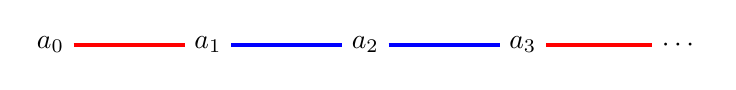
\begin{tikzpicture}
    \node at (0,0) (a0) {$a_0$};
\node at (2,0) (a1) {$a_1$};
\node at (4,0) (a2) {$a_2$};
\node at (6,0) (a3) {$a_3$};
\node at (8,0) (dd) {$\cdots$};
\draw[color=red, ultra thick] (a0) -- (a1);
\draw[color=blue, ultra thick] (a1) -- (a2);
\draw[color=blue, ultra thick] (a2) -- (a3);
\draw[color=red, ultra thick] (a3) -- (dd);
  \end{tikzpicture}\end{center}
  The subgraphs consisting of $a_0, a_3, \cdots$ and $a_1, a_2, \cdots$ are both
  monochromatic and at least one is infinite.\\\vspace{.25cm}
  The theorem can be extended to any finite number of colors.
\end{frame}

\begin{frame}
  \frametitle{Ramsey Theorem (finite)}
  \textbf{Ramsey Theorem} (finite version, Ramsey 1928): For any pair of positive integers $m$ and $n$,
    there exists an integer $k$ such that any complete graph on $k$ vertices with edges
    colored red and blue must contain either a monochromatic red complete subgraph on $m$
    vertices or a monochromatic blue complete subgraph on $n$ vertices.\\\vspace{.25cm}
  \textit{Proof Idea.} Let $R(m,n)=k$, the particular $k$ value required for the pair $m$ and
    $n$. Clearly $R(m,1)=R(1,n)=1$. Bound $R(m,n)$ inductively from above by
  $$R(m,n)\le R(m-1,n) + R(m,n-1).$$
\end{frame}

\begin{frame}[noframenumbering]
  \frametitle{Ramsey Theorem (finite)}
  \begin{center}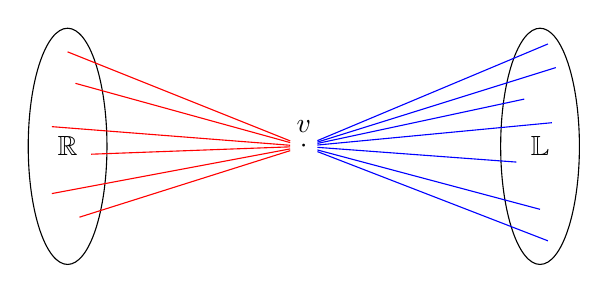
\begin{tikzpicture}
    \draw (0,0) ellipse (.5cm and 1.5cm);
\draw (6,0) ellipse (.5cm and 1.5cm);
\node at (0,0) (R) {$\mathbb{R}$};
\node at (6,0) (L) {$\mathbb{L}$};
\node at (3,0) (v) {$\cdot$}; \node at (3,.25) (label) {$v$};
\draw[color=red] (v) -- (0,1.2);
\draw[color=red] (v) -- (.1,.8);
\draw[color=red] (v) -- (-.2,.25);
\draw[color=red] (v) -- (.3,-.1);
\draw[color=red] (v) -- (-.2,-.6);
\draw[color=red] (v) -- (.15,-.9);
\draw[color=blue] (v) -- (6.1,1.3);
\draw[color=blue] (v) -- (6.2,1);
\draw[color=blue] (v) -- (5.8,.6);
\draw[color=blue] (v) -- (6.15,.3);
\draw[color=blue] (v) -- (5.7,-.2);
\draw[color=blue] (v) -- (6, -.8);
\draw[color=blue] (v) -- (6.1,-1.2);
  \end{tikzpicture}\end{center}
  \textbf{Case I}: $|\ \mathbb{R}\ |\ge R(m-1,n)$. $\mathbb{R}$ contains a red $K_{m-1}$ or
    a blue $K_n$, thus $G$ contains a red $K_m$ or a blue $K_n$.\\
  \textbf{Case II}: $|\ \mathbb{L}\ |\ge R(m,n-1)$. $\mathbb{L}$ contains a red $K_m$ or a
    blue $K_{n-1}$, thus $G$ contains a red $K_m$ or a blue $K_n$.\\
  Therefore $R(m,n)\le R(m-1,n)+R(m,n-1)$.
\end{frame}

\section{Definitions}

\begin{frame}
  \frametitle{Ramsey Numbers}
  Ramsey Theory deals with finding order amongst greater chaos. \\\vspace{.25cm} 
  Example: if we want to find a constellation of 10 stars forming a convex polygon where no three stars are collinear, how many stars do there need to be, to guarantee its occurrence? (The Happy Ending problem).  Ramsey numbers are a similar idea. 
\end{frame}

\begin{frame}[noframenumbering]
 \frametitle{Ramsey Numbers}
  \textbf{Ramsey Number}: The Ramsey number $R(n_1,....,n_c)=r$ is the least number such that if 
    the edges of a complete graph of order $r$ are colored with $c$ different 
    colors, then for some $i$ between 1 and $c$, it must contain a complete subgraph of order 
    $n_i$ whose edges are all color $i$. \\\vspace{.25cm}
  \textit{Motivating problem}: What is the minimum number of people you must invite to a party 
    to guarantee you will alway have 3 people who all know each other or 3 people who all do 
    not know each other? \\\vspace{.25cm} 
  In other words: What is R(3,3)?
\end{frame}

\begin{frame}
  \frametitle{Example: $R(3,3)$}
  \begin{center}
    \begin{minipage}[b]{.47\textwidth}
      \begin{center}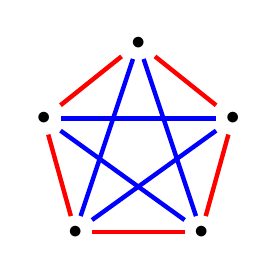
\begin{tikzpicture}[scale=.8]
  \node at (0,0) (n0) {$\bullet$};
  \node at (2,0) (n1) {$\bullet$};
  \node at (2.5,1.8) (n2) {$\bullet$};
  \node at (1,3) (n3) {$\bullet$};
  \node at (-.5,1.8) (n4) {$\bullet$};
  \draw [red, ultra thick] (n0) -- (n1);
  \draw [red, ultra thick] (n1) -- (n2);
  \draw [red, ultra thick] (n2) -- (n3);
  \draw [red, ultra thick] (n3) -- (n4);
  \draw [red, ultra thick] (n4) -- (n0);
  \draw [blue, ultra thick] (n0) -- (n2);
  \draw [blue, ultra thick] (n2) -- (n4);
  \draw [blue, ultra thick] (n4) -- (n1);
  \draw [blue, ultra thick] (n1) -- (n3);
  \draw [blue, ultra thick] (n3) -- (n0);
\end{tikzpicture}\end{center}
    \end{minipage}
    \begin{minipage}[b]{.47\textwidth}
      \begin{center}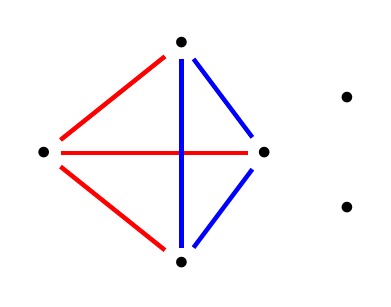
\begin{tikzpicture}[scale=.7]
  \node at (-1,3) (n0) {$\bullet$};
  \node at (1.5,1) (n1) {$\bullet$};
  \node at (1.5,5) (n2) {$\bullet$};
  \node at (3,3) (n3) {$\bullet$};
  \node at (4.5,2) (n4) {$\bullet$};
  \node at (4.5,4) (n5) {$\bullet$};
  \draw [red, ultra thick] (n0) -- (n1);
  \draw [red, ultra thick] (n0) -- (n2);
  \draw [red, ultra thick] (n0) -- (n3);
  \draw [blue, ultra thick] (n1) -- (n2);
  \draw [blue, ultra thick] (n1) -- (n3);
  \draw [blue, ultra thick] (n3) -- (n2);
\end{tikzpicture}\end{center}
    \end{minipage}
  \end{center}
  Since $K_5$ can be 2-colored without monochromatic triangles, $R(3,3)> 5$.
    Since $K_6$ cannot be colored without monochromatic triangles, $R(3,3)\le6$.
    Thus $R(3,3)=6$.
\end{frame}

\begin{frame}
  \frametitle{Bipartite Ramsey Numbers}
  \textbf{Two Color Bipartite Ramsey Number}: With 2 colors, red and blue, the bipartite 
    Ramsey number $b(m,n)$ is the least positive integer $b$ such that if the edges of $K(b,b)$ 
    are colored with red and blue, then there always exists a blue $K(m,m)$ or a red $K(n,n)$.\\
  \begin{minipage}[b]{.47\textwidth}
    \begin{center}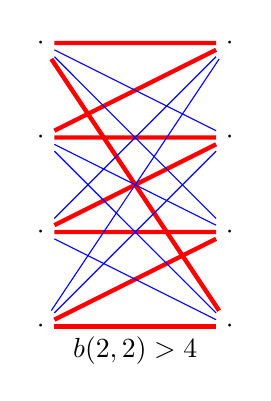
\begin{tikzpicture}[scale=.6]
  \node at (0,0) (v0) {$\cdot$};
  \node at (0,2) (v1) {$\cdot$};
  \node at (0,4) (v2) {$\cdot$};
  \node at (0,6) (v3) {$\cdot$};
  \node at (4,0) (u0) {$\cdot$};
  \node at (4,2) (u1) {$\cdot$};
  \node at (4,4) (u2) {$\cdot$};
  \node at (4,6) (u3) {$\cdot$};
  \foreach \x/\y in {v0/u0,v1/u1,v2/u2,v3/u3,v0/u1,v1/u2,v2/u3,v3/u0} \draw[color=red, ultra thick] (\x) -- (\y);
  \foreach \x/\y in {v0/u2,v0/u3,v1/u0,v1/u3,v2/u0,v2/u1,v3/u1,v3/u2} \draw[color=blue] (\x) -- (\y);
  \node at (2,-.5) (label) {$b(2,2)>4$};
%  \node at (5,0) (n0) {$\cdot$};
%  \node at (5,2) (n1) {$\cdot$};
%  \node at (5,4) (n2) {$\cdot$};
%  \node at (5,6) (n3) {$\cdot$};
%  \node at (8,0) (m0) {$\cdot$};
%  \node at (8,2) (m1) {$\cdot$};
%  \node at (8,4) (m2) {$\cdot$};
%  \node at (8,6) (m3) {$\cdot$};
%  \foreach \x/\y in {n0/m2,n0/m3,n1/m0,n1/m3,n2/m0,n2/m1,n3/m1,n3/m2} \draw[color=blue] (\x) -- (\y);
\end{tikzpicture}\end{center}

  \end{minipage}
  \begin{minipage}[b]{.47\textwidth}
    \begin{center}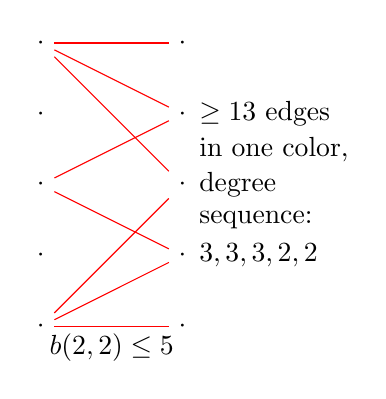
\begin{tikzpicture}[scale=.45]
  \node at (0,0) (v0) {$\cdot$};
  \node at (0,2) (v1) {$\cdot$};
  \node at (0,4) (v2) {$\cdot$};
  \node at (0,6) (v3) {$\cdot$};
  \node at (0,8) (v4) {$\cdot$};
  \node at (4,0) (u0) {$\cdot$};
  \node at (4,2) (u1) {$\cdot$};
  \node at (4,4) (u2) {$\cdot$};
  \node at (4,6) (u3) {$\cdot$};
  \node at (4,8) (u4) {$\cdot$};
  \foreach \x/\y in {v0/u0,v0/u1,v0/u2,v2/u1,v2/u3,v4/u4,v4/u3,v4/u2} \draw[color=red] (\x) -- (\y);
  \node[anchor=west] at (4.2,6) (t0) {$\ge13$ edges};
  \node[anchor=west] at (4.2,5) (t1) {in one color,};
  \node[anchor=west] at (4.2,4) (t2) {degree};
  \node[anchor=west] at (4.2,3) (t4) {sequence:};
  \node[anchor=west] at (4.2,2) (t3) {$3,3,3,2,2$};
  \node at (2,-.6) (lab) {$b(2,2)\le5$};
\end{tikzpicture}\end{center}

  \end{minipage}
\end{frame}

\begin{frame}[noframenumbering]
  \frametitle{Bipartite Ramsey Numbers}
  \textbf{Bipartite Ramsey Number}: The bipartite Ramsey number $b(n_1,...,n_k)$ is the 
    least positive integer $b$ such that any coloring of the edges of $K_{b,b}$, with $k$ colors 
    will result in a monochromatic copy of $K_{n_i,n_i}$, in the $i$-th color, for some $i$, $1\le 
    i \le k$.\\\vspace{.25cm} 
  If $n_i = m$ for all $i$, then we denote this number by $b_k(m)$.
\end{frame}

\begin{frame}
  \frametitle{Zarankiewicz Numbers}
  \textbf{Zarankiewicz Numbers}: The Zarankiewicz number $z(m,n;s,t)$ is the maximum 
    number of edges in a subgraph of $K_{m,n}$ that does not contain $K_{s,t}$ as a 
    subgraph. \\\vspace{.25cm}
  \textit{Special Case}: If $m=n$ and $s=t$, then we write $z(m,s)$ to denote the 
    number of edges in a subgraph of $K_{m,m}$ that does not contain $K_{s,s}$ as a 
    subgraph. \\\vspace{.25cm}
  \textit{Relation to Bipartite Ramsey Numbers}: For two colors, finding upper bounds for 
    Zarankiewicz numbers help provide upper bounds on bipartite Ramsey numbers.  
  $$z(b,m) + z(b,n) < b^2  \hspace{4 mm} \implies\hspace{4mm} b(m,n) \le b$$
  This relation can be extended to allow for more than two colors.
\end{frame}

\begin{frame}[noframenumbering]
  \frametitle{Zarankiewicz Numbers}
  \textit{Proof:} \\\vspace{.25cm}
    Let $z(b,m) = z_1$, and  $z(b,n) = z_2$ \\\vspace{.25cm}
    $K_{b,b}$ has $z_1$ red edges that does not contain a $K_{m,m}$ \\\vspace{.25cm}
    $K_{b,b}$ has $z_2$ blue edges that does not contain a $K_{n,n}$ \\\vspace{.25cm}
    We also know $K_{b,b}$ has $b^2$ edges \\\vspace{.25cm}
    If $z_1 + z_2 < b^2 \implies b(m,n) \le b$ \\\vspace{.50cm}
    Since if $b(m,n) = b+1$, $K_{b,b}$ will contain a red $K_{m,m}$ or a blue $K_{n,n}$ 
\end{frame}

\section{Problems of Interest}

\begin{frame}
  \frametitle{$b(2,5)$}
  It is known that $16\le b(2,5)\le19$. (Goddard et al. 2004) \\\vspace{.25cm} 
  \textit{Recall} that $b(2,5)$ is the smallest number of vertices in each partition of a complete 
    bipartite graph such that if the edges are colored red or blue we are guaranteed a 
    red $K_{2,2}$ or a blue $K_{5,5}$.\\\vspace{.25cm}
  We could improve the lower bound by finding edge colorings of $K_{16,16}$ which do not
    contain either of the forbidden subgraphs. Or we could improve the upper bound by 
    showing that all possible colorings of $K_{18,18}$ contain one of the forbidden 
    subgraphs. These graphs are not so large as to be computationally intractable.
\end{frame}


\begin{frame}
  \frametitle{$b_5(2)$}
  \textit{Recall} that $b_5(2)=b(2,2,2,2,2)$, the number of vertices in each partite set of a 
    complete bipartite graph such that any 5-coloring of the edges results in a monochromatic 
    4-cycle.\\\vspace{.25cm}
  \textbf{Problem of Interest}: Determining values for $b_k(2)$ seems to be a difficult problem. 
    The only known exact values are $b_2(2) = 5$, $b_3(2) = 11$, and $b_4(2) = 19$. \\
    \vspace{.25cm}
  \underline{Some Theorems}: (Dybizba$\acute{\text{n}}$ski, Dzido, Radziszowski, 2013) \\\vspace{.25cm} 
  \textit{Theorem 1}:  $b_k(2) \ge k^2 + 1$  \\\vspace{.25cm} 
  \textit{Theorem 2}: $b_k(2) \le k^2 + k -2$ \\\vspace{.25cm}
  \textit{Theorem 3}: $26 \le b_5(2) \le 28$ \\\vspace{.25cm}
  Possible conjecture for project: $b_5(2) = 28$
\end{frame}

\begin{frame}
  \frametitle{Readings}
  \begin{itemize}
    \item W.~Goddard, M.~A.~Henning and O.~R.~Oellermann, ``Bipartite Ramsey Numbers and 
      Zarankiewicz Numbers'', \textit{Elsevier Science} (2004).
    \item J.~Dybizba$\acute{\text{n}}$ski, T.~Dzido and S.~Radziszowski, ``On Some
      Zarankiewicz Numbers and Bipartite Ramsey Numbers for Quadrilateral''. Forthcoming (2013).
    \item R.~K.~Guy, ``A Many-Facetted Problem of Zarankiewicz'', \textit{The Many Facets of
      Graph Theory} (1969).
  \end{itemize}
\end{frame}

\begin{frame}
  \frametitle{Questions}
  \begin{center}
    {\Large Questions?}
  \end{center}
\end{frame}

\end{document}



